%package list
\documentclass{article}
\usepackage[top=3cm, bottom=3cm, outer=3cm, inner=3cm]{geometry}
\usepackage{graphicx}
\usepackage{url}
%\usepackage{cite}
\usepackage{hyperref}
\usepackage{array}
\usepackage{multicol}
\newcolumntype{x}[1]{>{\centering\arraybackslash\hspace{0pt}}p{#1}}
\usepackage{natbib}
\usepackage{pdfpages}
\usepackage{multirow}
\usepackage{float}
\usepackage[normalem]{ulem}
\usepackage{hyperref}
\useunder{\uline}{\ul}{}


%%%%%%%%%%%%%%%%%%%%%%%%%%%%%%%%%%%%%%%%%%%%%%%%%%%%%%%%%%%%%%%%%%%%%%%%%%%%
%%%%%%%%%%%%%%%%%%%%%%%%%%%%%%%%%%%%%%%%%%%%%%%%%%%%%%%%%%%%%%%%%%%%%%%%%%%%
\newcommand{\csemail}{vmachacaa@unsa.edu.pe}
\newcommand{\csdocente}{Vicente Machaca Arceda}
\newcommand{\cscurso}{Algoritmos y Estructura de Datos}
\newcommand{\csuniversidad}{Universidad Nacional de San Agustín}
\newcommand{\csescuela}{Maestría en Ciencia de la Computación}
\newcommand{\cspracnr}{02}
\newcommand{\cstema}{--}
%%%%%%%%%%%%%%%%%%%%%%%%%%%%%%%%%%%%%%%%%%%%%%%%%%%%%%%%%%%%%%%%%%%%%%%%%%%%
%%%%%%%%%%%%%%%%%%%%%%%%%%%%%%%%%%%%%%%%%%%%%%%%%%%%%%%%%%%%%%%%%%%%%%%%%%%%


\usepackage[english,spanish]{babel}
\usepackage[utf8]{inputenc}
\AtBeginDocument{\selectlanguage{spanish}}
\renewcommand{\figurename}{Figura}
\renewcommand{\refname}{Referencias}
\renewcommand{\tablename}{Tabla} %esto no funciona cuando se usa babel
\AtBeginDocument{%
	\renewcommand\tablename{Tabla}
}

\usepackage{fancyhdr}
\pagestyle{fancy}
\fancyhf{}
\setlength{\headheight}{30pt}
\renewcommand{\headrulewidth}{1pt}
\renewcommand{\footrulewidth}{1pt}
\fancyhead[L]{\raisebox{-0.2\height}{
\includegraphics[width=3cm]{img/logo_unsa}}}
\fancyhead[C]{}
\fancyhead[R]{\fontsize{7}{7}\selectfont	\csuniversidad \\ \csescuela \\ \textbf{\cscurso} }
\fancyfoot[L]{MSc. Vicente Machaca}
\fancyfoot[C]{\cscurso}
\fancyfoot[R]{Página \thepage}


\begin{document}
	
	\vspace*{10px}
	
	\begin{center}	
		\fontsize{17}{17} \textbf{ Práctica \cspracnr}
	\end{center}
	%\centerline{\textbf{\underline{\Large Título: Informe de revisión del estado del arte}}}
	%\vspace*{0.5cm}
	

	\begin{table}[h]
		\begin{tabular}{|x{4.7cm}|x{4.8cm}|x{4.8cm}|}
			\hline
			\textbf{DOCENTE} & \textbf{CARRERA}  & \textbf{CURSO}   \\
			\hline
			\csdocente & \csescuela & \cscurso    \\
			\hline
		\end{tabular}
	\end{table}	
	
	
	\begin{table}[h]
		\begin{tabular}{|x{4.7cm}|x{4.8cm}|x{4.8cm}|}
			\hline
			\textbf{PRÁCTICA} & \textbf{TEMA}  & \textbf{DURACIÓN}   \\
			\hline
			\cspracnr & \cstema &  -  \\
			\hline
		\end{tabular}
	\end{table}
	
	
	\section{Datos de los estudiantes}
	\begin{itemize}
		\item Grupo: 2
		\item Integrantes:
		\begin{itemize}
			\item EDER ALONSO AMPUERO ATAMARI
			\item HOWARD FERNANDO ARANZAMENDI MORALES
            \item JOSE EDISON PEREZ MAMANI
            \item HENRRY IVAN ARIAS MAMANI
		\end{itemize}		
	\end{itemize}
        \section{Url Github }
      Repositorio Github: \href{https://github.com/hAriasm/Practica2_ayed}{Práctica 2}  
	\section{Algoritmo de Ordenamiento}\label{sec:ejercicios}



     \subsection{BTree}
    \paragraph{}
    El Merge Sort es un algoritmo recursivo bastante eficiente para ordenar un array, que tiene un orden de complejidad O(nlogn) al igual que Quick Sort. fue desarrollado en 1945 por John Von Neumann.

    El Merge Sort está basado en la técnica de diseño de algoritmos Divide y Vencerás, esta técnica consiste en dividir el problema a resolver en sub problemas del mismo tipo que a su vez se dividirán, mientras no sean suficientemente  pequeños o triviales.
    \begin{figure}[h!]
        \centering
        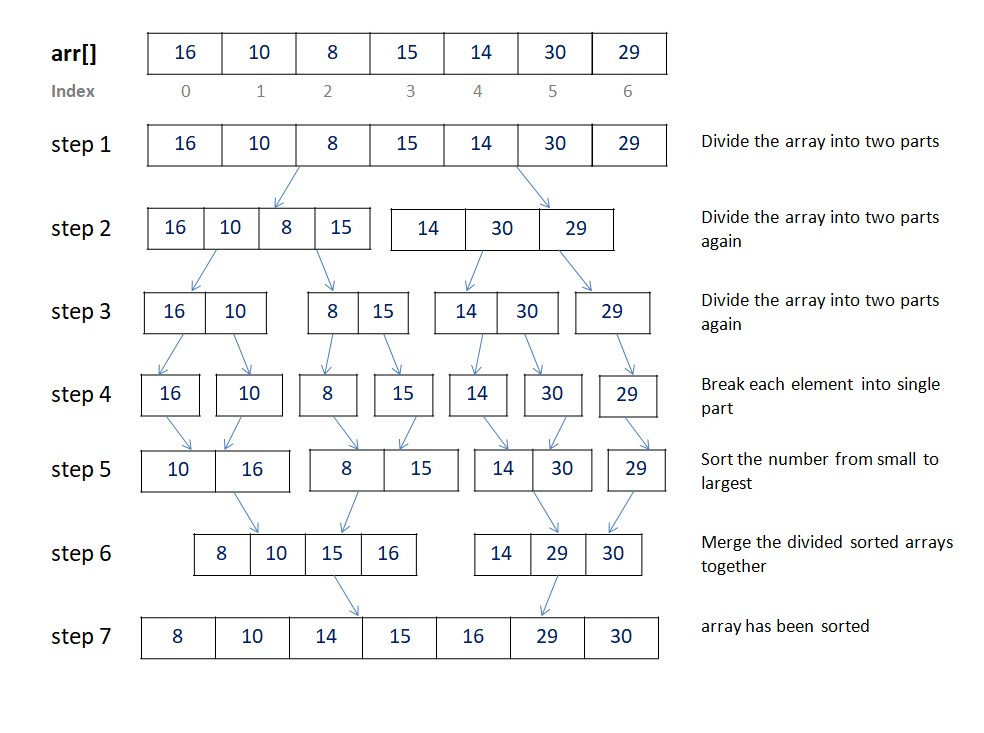
\includegraphics[width=12cm]{img/mergesort.png}
        \caption{Estrategia que sigue algoritmo para ordenar una secuencia S de n elementos}
        \label{fig:mergesort}
    \end {figure}
    \begin{itemize}
        \item Si S tiene uno o ningún elemento, está ordenada.
        \item Si S tiene al menos dos elementos se divide en dos secuencias S1 y S2.
        \item S1 contiene los primeros n/2 elementos y S2 los restantes.
        \item Ordenar S1 y S2, aplicando recursivamente este procedimiento
        \item Mezclar S1 y S2 en S, de forma que ya S1 y S2 estén ordenados
        \item Veamos ahora como sería la estrategia para mezclar las secuencias:
    \end{itemize}
    \paragraph {}
   
    \subsection{AVL}
        \paragraph {}
        Quicksort ha sido históricamente el algoritmo genérico \label[aaaa]{quickSortPython}de ordenamiento más rápido conocido en la práctica. Es un algoritmo recursivo del tipo “divide y vencerás”, es fácil de implementar, que permite, en promedio, ordenar n elementos en un tiempo proporcional a n log n.
        \paragraph {}
        La idea básica es ordenar una lista siguiendo los pasos siguientes: se escoge un elemento arbitrario de la lista y se forman tres grupos; el primer grupo, tiene los elementos menores a aquel que se escogió; el segundo, los elementos iguales que el escogido; y el tercero, tiene los elementos más grandes. De forma recursiva, se ordenan el primer y el tercer grupo; luego, se concatenan todos los grupos.
        \paragraph {}
        Este método fue creado por el científico británico Charles Antony Richard Hoare, también conocido como Tony Hoare en 1960, su algoritmo Quicksort es el algoritmo de ordenamiento más ampliamente utilizado en el mundo.
           \begin{figure}[h!]
            \centering
            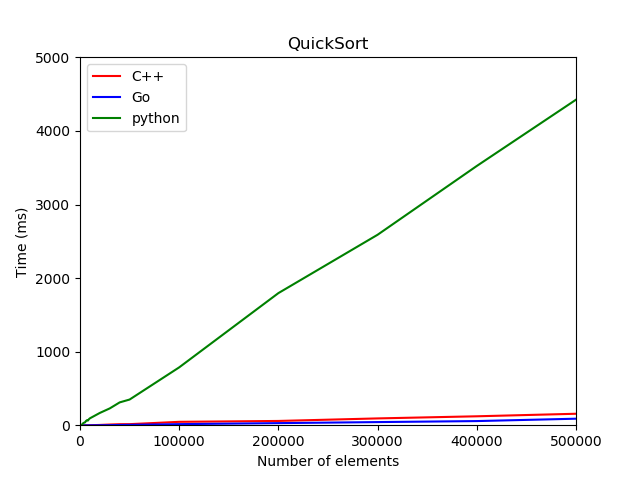
\includegraphics[width=12cm]{img/QuickSort_1.png}
            \caption{Estrategia que sigue algoritmo para ordenar una secuencia S de n elementos}
            \label{fig:mergesort}
        \end {figure}




   \section{Conclusiones}
   \begin{itemize}
     \item  En las pruebas realizadas para el Algoritmo Quick Sort, se obtuvo tiempos de ejecución menores para el código desarrollado en lenguaje de programación Golang, y tiempos de mayor valor en la ejecución del código en lenguaje de programación Python.
     \item	Se observó que, para tamaños de entrada menores a 10 000 datos, los tiempos de ejecución son inconsistentes, al ejecutar el código del algoritmo Quick Sort en lenguaje Golang, presentándose en reiteradas oportunidades valores de cero.
     \item	En la ejecución del algoritmo Quick Sort, los valores de desviación estándar son mayores al ejecutar el código en lenguaje Python, y presentan valores menores al usar el código en C++. Para las pruebas realizadas en Python se observa que los valores de desviación estándar van en aumento respecto al tamaño de la entrada, en el caso del lenguaje Golang y C++, estos valores se incrementan desde 100 000 y 20 000 datos, respectivamente.
     \item  Los programas en lenguaje compilado (C++) presenta un mejor desempeño en cuanto se presenta mayor cantidad de datos que un programa en lenguaje interpretado (Python)
   \end{itemize}

   \section{Referencias}

\end{document} 